\let\negmedspace\undefined
\let\negthickspace\undefined
\documentclass[journal]{IEEEtran}
\usepackage[a5paper, margin=10mm, onecolumn]{geometry}
\usepackage{lmodern} % Ensure lmodern is loaded for pdflatex
 % Include tfrupee package
\setlength{\headheight}{1cm} % Set the height of the header box
\setlength{\headsep}{0mm}     % Set the distance between the header box and the top of the text
\usepackage{enumitem}
\usepackage{gvv-book}
\usepackage{gvv}
\usepackage{cite}
\usepackage{amsmath,amssymb,amsfonts,amsthm}
\usepackage{algorithmic}
\usepackage{graphicx}
\usepackage{textcomp}
\usepackage{xcolor}
\usepackage{txfonts}
\usepackage{listings}
\usepackage{enumitem}
\usepackage{mathtools}
\usepackage{gensymb}
\usepackage{comment}
\usepackage[breaklinks=true]{hyperref}
\usepackage{tkz-euclide} 
\usepackage{listings}
% \usepackage{gvv}                                        
\def\inputGnumericTable{}                                 
\usepackage[latin1]{inputenc}                                
\usepackage{color}                                            
\usepackage{array}                                            
\usepackage{longtable}                                       
\usepackage{calc}                                             
\usepackage{multirow}                                         
\usepackage{hhline}                                           
\usepackage{ifthen}                                           
\usepackage{lscape}
\begin{document}

\bibliographystyle{IEEEtran}
\vspace{3cm}

\title{3-3-9}
\author{AI24BTECH11008- Sarvajith
}
% \maketitle
% \newpage
% \bigskip
{\let\newpage\relax\maketitle}

\renewcommand{\thefigure}{\theenumi}
\renewcommand{\thetable}{\theenumi}
\setlength{\intextsep}{10pt} % Space between text and floats
\numberwithin{equation}{enumi}
\numberwithin{figure}{enumi}
\renewcommand{\thetable}{\theenumi}
\textbf{Question: }\\
Draw an isosceles triangle ABC in which BC = 5.5cm and altitude AL = 5.3cm. \\
\textbf{Solution: }\\
\renewcommand{\tablename}{TABLE 1}
\begin{table}[h!]    
\centering
 \begin{tabular}{|c|c|}
\hline
\textbf{lengths} & \textbf{values}\\
\hline
\textbf{BC} & 5.5cm\\
\hline
\textbf{AL} & 5.3cm\\
\hline
\end{tabular}

\caption{values of lengths of triangle}
 \label{tab1-1.2-18-1}
\end{table}
The vertices of the above triangle are given by:
\begin{align}
    \textbf{A} &= \myvec{a\\b} \label{eq. 3-3-9.1}\\
    \textbf{B} &= \myvec{0\\0}\label{eq. 3-3-9.2}\\
    \textbf{C} &= \myvec{a\\0}\label{eq. 3-3-9.3}
\end{align}
\begin{align}
b &= c
\end{align}
as AL perpendicularly bisect BC, triangle ALB is rightangled \\
\begin{align}
\therefore AL^2 + \frac{a^2}{4} &= b^2\\
b&=c=5.97\\
\cos B &= \frac{a}{2b} = 0.46
\end{align}
Where a,b,c are BC,AB,AC respectively and B is the angle formed by the side AB and BC.\\
\begin{align*}
	a+b+c&=K\\
	-a+b\cos(C)+c\cos(B)&=0\\
	b\sin(C)-c\sin(B)&=0\\
\end{align*}
It results in the following matrix equation
\begin{align*}
  \myvec{1 & 1 & 1\\-1 & \cos(C) & \cos(B)\\0 & \sin(C) & -\sin(B)}\times\myvec{a\\b\\c}&=K\myvec{1\\0\\0}
\end{align*}
as the given triangle is iscosceles $\angle B = \angle C$\\
We can find all the side lengths by solving the above matrix equation where $x=\frac{a}{K}$, $y=\frac{b}{K}$, and $z=\frac{c}{K}$.\\
the augmented matrix will be\\
\begin{align*}
	\myvec{1 & 1 & 1 & 1\\ -1 & \cos B & \cos B & 0\\ 0 & \sin C & -\sin C & 0}\xleftrightarrow[]{R_3 \leftarrow {\frac{R_3}{\sin C}}}\myvec{1 & 1 & 1 & 1\\ -1 & \cos B & \cos B & 0\\ 0 & 1 & -1 & 0}\\
	\xleftrightarrow[]{R_2 \leftarrow {R_2+R_1}} \myvec{1 & 1 & 1 & 1\\ 0 & 1 + \cos B & 1 + \cos B & 1\\ 0 & 1 & -1 & 0}\\
	\xleftrightarrow[]{R_2 \leftarrow {\frac{R_2}{1 + \cos B}}}\myvec{1 & 1 & 1 & 1\\ 0 & 1 & 1 & \frac{1}{1 + \cos B}\\ 0 & 1 & -1 & 0}\\
	\xleftrightarrow[]{R_1 \leftarrow {R_1-R_2}}\myvec{1 & 0 & 0 & 1 - \frac{1}{1 + \cos B}\\ 0 & 1 & 1 & \frac{1}{1 + \cos B}\\0 & 1 & -1 & 0}\\
	\xleftrightarrow[]{R_3 \leftarrow {-R_3+R_2}}\myvec{1 & 0 & 0 & 1 - \frac{1}{1 + \cos B}\\ 0 & 1 & 1 & \frac{1}{1 + \cos B}\\ 0 & 0 & 2 & \frac{1}{1 + \cos B}}\\
	\xleftrightarrow[]{R_3 \leftarrow {\frac{R_3}{2}}}\myvec{1 & 0 & 0 & 1 - \frac{1}{1 + \cos B}\\ 0 & 1 & 1 & \frac{1}{1 + \cos B}\\ 0 & 0 & 1 & \frac{1}{2\brak{1 + \cos B}}}\\
	\xleftrightarrow[]{R_2 \leftarrow {R_2-R_3}}\myvec{1 & 0 & 0 & 1 - \frac{1}{1+\cos B}\\ 0 & 1 & 0 & \frac{1}{2\brak{1 + \cos B}}\\ 0 & 0 & 1 & \frac{1}{2\brak{1 + \cos B}}}\\
\end{align*}
The values of $x$,$y$,$z$ are
\begin{align}
\frac{a}{K} &= 1 - \frac{1}{1+\cos B}\label{eq. 3-3-9.4}\\
\frac{b}{K} &= \frac{1}{2\brak{1 + \cos B}}\label{eq. 3-3-9.5}\\
\frac{c}{K} &= \frac{1}{2\brak{1 + \cos B}}\label{eq. 3-3-9.6}
\end{align}
Substituting  the values of a,b,c in \ref{eq. 3-3-9.1}, \ref{eq. 3-3-9.2} and \ref{eq. 3-3-9.3}. Gives the coordinates. 
\begin{align*}
     \textbf{A}&=\myvec{2.75\\5.3}\\
     \textbf{B}&=\myvec{0\\0}\\
     \textbf{C}&=\myvec{5.5\\0}
\end{align*}


\begin{figure}[h!]
\centering
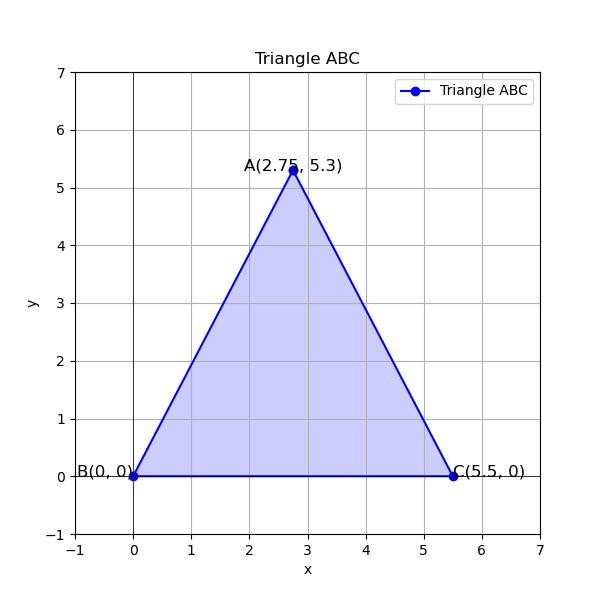
\includegraphics[width=0.7\columnwidth]{figs/Figure_1.png}
\caption{plot for isosceles triangle}
 \label{fig. 3-3-9-1}
\end{figure}
\end{document}

